% Hlavicka pro protokoly z fyzikalniho praktika.
% Verze pro: LaTeX
% Verze hlavicky: 22. 2. 2007
% Autor: Ustav fyziky kondenzovanych latek
% Ke stazeni: www.physics.muni.cz/ufkl/Vyuka/
% Licence: volne k pouziti, nejlepe k vcasnemu odevzdani protokolu z Vaseho mereni.

\documentclass[a4paper,11pt]{article}

% Kodovani (cestiny) v dokumentu: utf-8
%\usepackage[cp1250]{inputenc}	% Omezena stredoevropska kodova stranka, pouze MSW.
\usepackage[utf8]{inputenc}	% Doporucujeme pouzivat UTF-8 (unicode).
\usepackage[T1]{fontenc}
\usepackage{lmodern}

%%% Nemente:
\usepackage[margin=2cm]{geometry}
\newtoks\jmenopraktika \newtoks\jmeno \newtoks\datum
\newtoks\obor \newtoks\skupina \newtoks\rocnik \newtoks\semestr
\newtoks\cisloulohy \newtoks\jmenoulohy
\newtoks\tlak \newtoks\teplota \newtoks\vlhkost
\usepackage{amsmath}
\usepackage{mathtools}
\usepackage{graphicx}
\usepackage{multirow}

\usepackage{pgfplotstable} 
\usepackage{booktabs}

\graphicspath{ {./images/} }
%%% Nemente - konec.


%%%%%%%%%%% Doplnte pozadovane polozky:

\jmenopraktika={Fyzikální praktikum 3}  % nahradte jmenem vaseho predmetu
\jmeno={Artem Gorodilov}            % nahradte jmenem mericiho
\datum={4. ~března 2024}  % nahradte mistem a datem mereni
\obor={Astrofyzika}                     % nahradte zkratkou vami studovaneho oboru
\skupina={Po 14:00}            % nahradte dobou vyuky vasi seminarni skupiny
\rocnik={II}                  % nahradte rocnikem, ve kterem studujete
\semestr={II}                 % nahradte semestrem, ve kterem studujete

\cisloulohy={B}               % nahradte cislem merene ulohy
\jmenoulohy={Milikanův experiment}             % nahradte jmenem merene ulohy

\tlak={979}                   % nahradte tlakem pri mereni (v hPa)
\teplota={21.4}               % nahradte teplotou pri mereni (ve stupnich Celsia)
\vlhkost={46}               % nahradte vlhkosti vzduchu pri mereni (v %)

%%%%%%%%%%% Konec pozadovanych polozek.


%%%%%%%%%%% Uzitecne balicky:
\usepackage[czech]{babel}
\usepackage{graphicx}
\usepackage{amsmath}
\usepackage{xspace}
\usepackage{url}
\usepackage{indentfirst}
\usepackage{listings}
\usepackage{subcaption}
\usepackage{caption}
\usepackage{tabularx}
\usepackage[labelformat=parens,labelsep=quad,skip=3pt]{caption}

%%%%%% Zamezeni parchantu:
\widowpenalty 10000 \clubpenalty 10000 \displaywidowpenalty 10000
%%%%%% Parametry pro moznost vsazeni vetsiho poctu obrazku na stranku
\setcounter{topnumber}{3}	  % max. pocet floatu nahore (specifikace t)
\setcounter{bottomnumber}{3}	  % max. pocet floatu dole (specifikace b)
\setcounter{totalnumber}{6}	  % max. pocet floatu na strance celkem
\renewcommand\topfraction{0.9}	  % max podil stranky pro floaty nahore
\renewcommand\bottomfraction{0.9} % max podil stranky pro floaty dole
\renewcommand\textfraction{0.1}	  % min podil stranky, ktery musi obsahovat text
\intextsep=8mm \textfloatsep=8mm  %\intextsep pro ulozeni [h] floatu a \textfloatsep pro [b] or [t]

% Tecky za cisly sekci:
\renewcommand{\thesection}{\arabic{section}.}
\renewcommand{\thesubsection}{\thesection\arabic{subsection}.}
% Jednopismenna mezera mezi cislem a nazvem kapitoly:
\makeatletter \def\@seccntformat#1{\csname the#1\endcsname\hspace{1ex}} \makeatother

\begin{document}

\thispagestyle{empty}

{
\begin{center}
\sf 
{\Large Ústav fyzikální elektroniky PřF MU} \\
\bigskip
{\huge \bfseries FYZIKÁLNÍ PRAKTIKUM} \\
\bigskip
{\Large \the\jmenopraktika}
\end{center}

\bigskip

\sf
\noindent
\setlength{\arrayrulewidth}{1pt}
\begin{tabular*}{\textwidth}{@{\extracolsep{\fill}} l l}
\large {\bfseries Zpracoval:}  \the\jmeno & \large  {\bfseries Naměřeno:} \the\datum\\[2mm]
\large  {\bfseries Obor:} \the\obor  \hspace{40mm}  {\bfseries Skupina:} \the\skupina %
%{\bfseries Ročník:} \the\rocnik \hspace{5mm} {\bfseries Semestr:} \the\semestr  
&\large {\bfseries Testováno:}\\
\\
\hline
\end{tabular*}
}

\bigskip

{
\sf
\noindent \begin{tabular}{p{3cm} p{0.6\textwidth}}
\Large  Úloha č. {\bfseries \the\cisloulohy:} \par
\smallskip
% $T=\the\teplota$~$^\circ$C \par
% $p=\the\tlak$~hPa \par
% $\varphi=\the\vlhkost$~\%
&\Large \bfseries \the\jmenoulohy  \\[2mm]
\end{tabular}
}

\vskip10pt
    \begin{minipage}[t]{0.5\textwidth} 
        \section{Zadání}    
            \begin{enumerate}
                \item Zmeřit velikost elementárního náboje pomocí rychlostí padající a stoupající olejové kapičky v homogenním elektrickém poli. Provest merení rychlostí alespon padesáti kapiček pro různé hodnoty napětí mezi elektrodami.
            \end{enumerate}
        \section{Teorie}
            Milikanův experiment je experimentální metoda pro měření elementárního náboje. V experimentu se měří rychlost kapiček oleje, které padají nebo stoupají v elektrickém poli. Kapičky jsou získány rozprašováním oleje v elektrickém poli. Kapičky jsou zrychlovány elektrickým polem a jejich rychlost je měřena. Z měření rychlosti kapiček lze určit náboj kapičky a tím i elementární náboj.
            \par Rovnovážná rychlost kapičky $\upsilon_1$ která přitahována elektrickým polem ke spodní elektrodě je dána vztahem:
            \begin{equation}
                \frac{4}{3} \pi r^3 \rho g + |q| E = \frac{4}{3} \pi r^3 \rho_{vz} g + 6 \pi \eta r \upsilon_1
            \end{equation}
            kde $r$ je poloměr kapičky, $\rho$ je hustota oleje, $\rho_{vz}$ je hustota vzduchu, $g$ je tíhové zrychlení, $\eta$ je dynamická viskozita vzduchu, $E$ je intenzita elektrického pole a $q$ je náboj kapičky.
            \par Rovnovážná rychlost kapičky $\upsilon_2$ která je odpuzována elektrickým polem od spodní elektrody a letí nahoru je dána vztahem:
            \begin{equation}
                \frac{4}{3} \pi r^3 \rho_{vz} g + |q| E = \frac{4}{3} \pi r^3 \rho g - 6 \pi \eta r \upsilon_2
            \end{equation}
            \par Z těchto dvou vztahů lze vyjádřit poloměr kapičky $r$ a náboj kapičky $q$:
            \begin{equation}
                r = \sqrt{\frac{9 \eta (\upsilon_1 - \upsilon_2)}{4 g (\rho - \rho_{vz})}}
            \end{equation}
    \end{minipage}
    \hspace{10pt} 
    \begin{minipage}[t]{0.5\textwidth} 
            \begin{equation}
                |q| = 3 \pi \eta r \frac{\upsilon_1 + \upsilon_2}{E} ~ , ~ E = \frac{U}{d}
            \end{equation}
            kde $U$ je napětí mezi elektrodami a $d$ je vzdálenost mezi elektrodami.
            \par Kapka může nést náboj $q = n \cdot e$, kde $n$ je počet nábojů a $e$ je elementární náboj. Naboj kapiček se shlukuje do skupin, které mají náboj $q = n \cdot e$. 
            \par Můžeme určit $n-1$ rozdílů průměrného náboje kapiček dvou sousedních shluků ($q_{i+1} - q_i$):
            \begin{equation}
                \frac{1}{n-1} \sum_{i=1}^{n-1} (q_{i+1} - q_i) = \frac{q_n - q_1}{n-1}
            \end{equation}
        \section{Měření}
            Měření probíha nasledovně:
            \begin{enumerate}
                \item Nastavíme napětí mezi elektrodami na hodnotu $U$.
                \item Rozprašujeme olejové kapičky do komůrky.
                \item Urcíme rychlost kapiček, pomicí skriptu v pythonu\cite{vitek}.
                \item Opakujeme měření pro různé hodnoty napětí mezi elektrodami.
            \end{enumerate}
            \par Měření bylo provedeno pro napětí mezi elektrodami $U = 300$ V, $U = 400$ V, $U = 500$ V a $U = 600$ V.
            \par Tabulkové hodnoty použité při výpočtu:
            \begin{center}
                \begin{tabular}{ll}
                    $g$ = 9.81 m/s$^2$ \\
                    $\rho$ = 1030 kg/m$^3$ \\
                    $\rho_{vz}$ = 1.293 kg/m$^3$\cite{density} \\
                    $\eta$ = 1.81 $\cdot 10^{-5}$ Pa$\cdot$s\cite{viscosity} \\
                    $d$ = 2.5 mm \\
                \end{tabular}
            \end{center}
    \end{minipage}
\newpage
    \begin{minipage}[t]{0.5\textwidth}   
            Pomocí skriptu v pythonu jsme analyzovali videa pořízená během měření. Pro analýzu byly použity následující parametry funkcí skriptu: 
            \vspace{5pt}
            \par \texttt{kapkatrack.py --min-b 100 data/*.mpg}
            \vspace{5pt}
            \par \texttt{kapkal.py data/*.mpg --save-plots -f 5 -x 50 --fit-std-threshold 50}
            \vspace{5pt}
            \par Ze získaných rychlostí $\upsilon_1$ a $\upsilon_2$ jsme pak vypočítali poloměry kapek $r$ a jejich náboj $q$ pomocí vzorců (3) a (4). 
            \par Poté jsme zjistili intervaly, ve kterých se nacházejí skupiny nábojů. Výsledky jsou uvedeny na obrázku (1).
            \par Na základě toho jsme náboje rozdělili do skupin a určili jejich stupeň ionizace. Poté jsme tyto údaje vynesli do grafu a provedli lineární fit. Výsledky jsou uvedeny na obrázku (2).
            \par Z toho jsme získali hodnotu elementárního náboje $q_0$: 
            \begin{center}
                $q_0$ = 1.56(3) $\cdot 10^{-19}$ C
            \end{center}

            \vspace{10pt}           
            \par \centering
            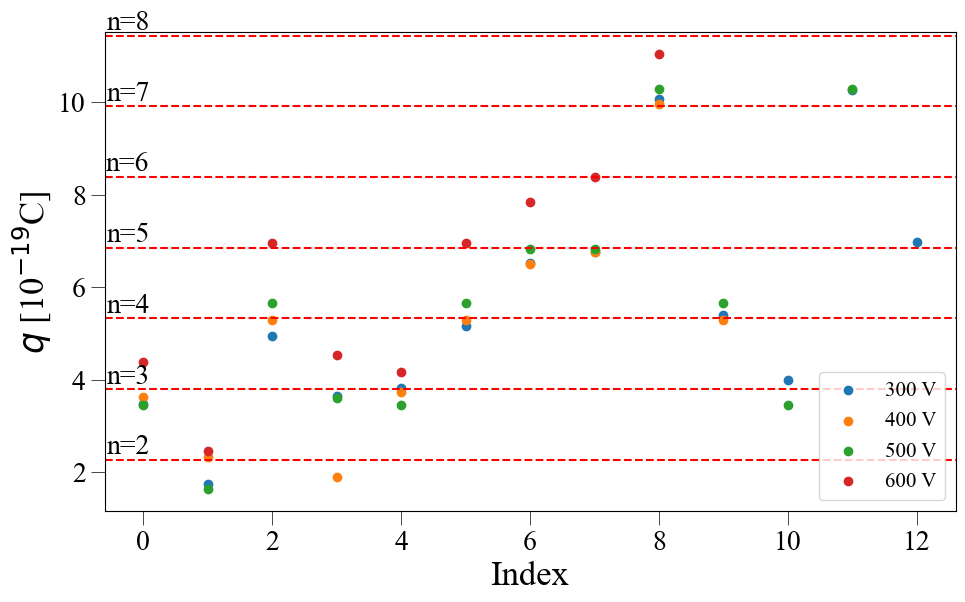
\includegraphics[scale=0.35]{lvl}
            \captionsetup{justification=centering, font=footnotesize}
            \captionof{figure}{Rozdělení nábojů podle stupně ionizace.}
            \label{fig:lvl}
            \vspace{10pt}
            \raggedright 

            \par Výsledky měření jsou v tabulce (1), (2), (3) a (4).
            \par K výpočtu veličin a jejich nejistot byla použita knihovna Uncertinties pro Python \cite{uncertainties}.
    \end{minipage}
    \hspace{10pt}
    \begin{minipage}[t]{0.5\textwidth} 
            \vspace{10pt}           
            \par \centering
            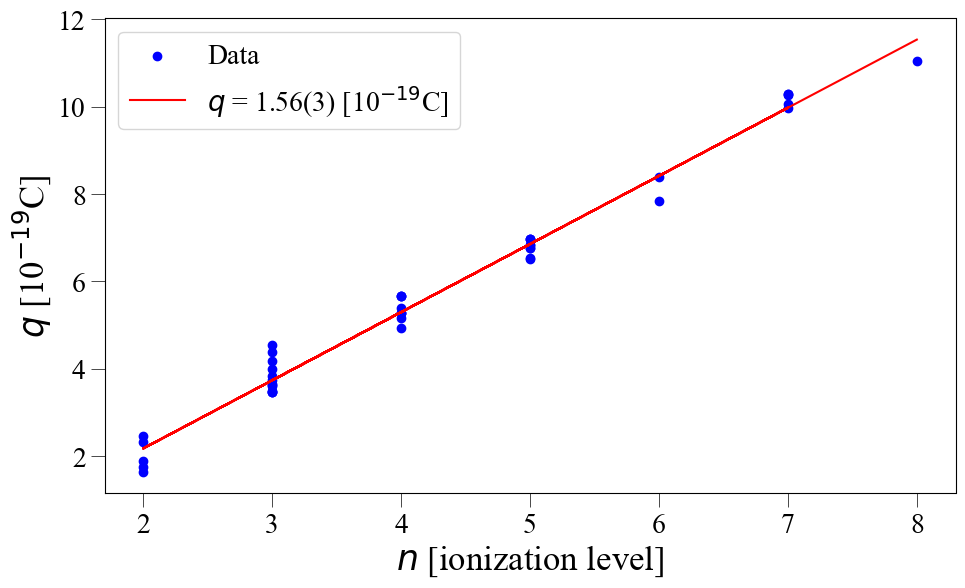
\includegraphics[scale=0.35]{q}
            \captionsetup{justification=centering, font=footnotesize}
            \captionof{figure}{Zavislost náboje na stupni ionizace.}
            \label{fig:q}
            \vspace{10pt}
            \raggedright 
            
            \par Chyby byly rozšířeny o Studentův koeficient (2-Tail Confidence Level) s ohledem na stupně volnosti pro každou hodnotu, pro interval spolehlivosti 68.27\%.
        \section{Závěr}  
            Jsme určili hodnotu elementárního náboje $q_0$ = 1.56(3) $\cdot 10^{-19}$ C. Tato hodnota je v souladu s tabulkovou hodnotou elementárního náboje $q_0$ = 1.602 $\cdot 10^{-19}$ C. 
            \par Rozdíl může být způsoben nepřesností při měření rychlosti kapek pomocí skriptu Python. To zase mohlo být způsobeno tím, že jsme během měření měnili zaostření, což zase mohlo změnit jas pozadí. Vzhledem k tomu, že skript odečítá pozadí od každého snímku, aby získal mapu pohybu kapek, je možné, že spolu s pozadím bylo odečteno i mnoho kapek, které byly rozostřené nebo nebyly dostatečně jasné. 
            \par Bohužel, nepodařilo získat větší počet kapek kvůli zvláštnostem experimentu a jeho zpracování skriptem. 
    \end{minipage}
    \vspace{20pt}

    \begin{thebibliography}{9}
        \bibitem{vitek} 
            Tomáš Vítek, Available online: \url{https://is.muni.cz/auth/el/sci/jaro2024/F4210/um/fp3_-_zpracovani_obrazu/Millikan-zpracovani_obrazu-python.zip}
        \bibitem{density}
            Air Mass/Density, NASA Earthdata, Available online: \url{https://www.earthdata.nasa.gov/topics/atmosphere/atmospheric-pressure/air-mass-density}
        \bibitem{viscosity}
            Viscosity of Air, Dynamic and Kinematic, Engineers Edge, Available online: \url{https://www.engineersedge.com/physics/viscosity_of_air_dynamic_and_kinematic_14483.htm}
        \bibitem{uncertainties}
            Uncertainties, Available online: \url{https://pypi.org/project/uncertainties}
    \end{thebibliography}
        
\newpage
        \section{Přílohy}   
            \begin{center}
                \subsection{Tabulka (1) naměřených a vypočtených hodnot pro $U$ = 300 V} 
                    \pgfplotstabletypeset[
                        col sep=comma, % Defines the separator, comma for CSV
                        string type, % Treats columns as strings (not math mode)
                        every head row/.style={before row=\toprule,after row=\midrule},
                        every last row/.style={after row=\bottomrule},
                        columns/v1/.style={column name=\upsilon_1 [10^{-4} m/s]},
                        columns/v2/.style={column name=\upsilon_2 [10^{-4} m/s]},
                        columns/r/.style={column name=r [10^{-7} m]},
                        columns/q/.style={column name=q [10^{-19} C]},
                    ]{data/U_300.csv} 
            \end{center}
            \begin{center}
                \subsection{Tabulka (2) naměřených a vypočtených hodnot pro $U$ = 400 V} 
                    \pgfplotstabletypeset[
                        col sep=comma, % Defines the separator, comma for CSV
                        string type, % Treats columns as strings (not math mode)
                        every head row/.style={before row=\toprule,after row=\midrule},
                        every last row/.style={after row=\bottomrule},
                        columns/v1/.style={column name=\upsilon_1 [10^{-4} m/s]},
                        columns/v2/.style={column name=\upsilon_2 [10^{-4} m/s]},
                        columns/r/.style={column name=r [10^{-7} m]},
                        columns/q/.style={column name=q [10^{-19} C]},
                    ]{data/U_400.csv} 
            \end{center}
            \begin{center}
                \subsection{Tabulka (3) naměřených a vypočtených hodnot pro $U$ = 500 V} 
                    \pgfplotstabletypeset[
                        col sep=comma, % Defines the separator, comma for CSV
                        string type, % Treats columns as strings (not math mode)
                        every head row/.style={before row=\toprule,after row=\midrule},
                        every last row/.style={after row=\bottomrule},
                        columns/v1/.style={column name=\upsilon_1 [10^{-4} m/s]},
                        columns/v2/.style={column name=\upsilon_2 [10^{-4} m/s]},
                        columns/r/.style={column name=r [10^{-7} m]},
                        columns/q/.style={column name=q [10^{-19} C]},
                    ]{data/U_500.csv}
            \end{center}
            \begin{center}
                \subsection{Tabulka (4) naměřených a vypočtených hodnot pro $U$ = 600 V} 
                    \pgfplotstabletypeset[
                        col sep=comma, % Defines the separator, comma for CSV
                        string type, % Treats columns as strings (not math mode)
                        every head row/.style={before row=\toprule,after row=\midrule},
                        every last row/.style={after row=\bottomrule},
                        columns/v1/.style={column name=\upsilon_1 [10^{-4} m/s]},
                        columns/v2/.style={column name=\upsilon_2 [10^{-4} m/s]},
                        columns/r/.style={column name=r [10^{-7} m]},
                        columns/q/.style={column name=q [10^{-19} C]},
                    ]{data/U_600.csv}
            \end{center}
\end{document}